\documentclass[12pt]{article}
%compile using XeLaTeX
\usepackage{diary_style}
\setlength{\footskip}{\paperheight
  -(0.75in+\voffset+\topmargin+\headheight+\headsep+\textheight)
  -0.75in}

%\fontspec{Times New Roman}

\DeclareMathOperator{\di}{d\!}
\newcommand*\Eval[3]{\left.#1\right\rvert_{#2}^{#3}}

\begin{document}

%\doublespacing
\vspace{1.0 \baselineskip}

\begin{flushright}
	Alexander Caines\\
	MATH-310\\
	4-15-2021\\
\end{flushright}

\begin{center}
	\textbf{\underline{FINAL}}
\end{center}


%\vspace{0.5 \baselineskip}

\begin{enumerate}
	\item[1.] Let the null hypothesis be that there is no difference in death rates for men and women, 
		while the alternative hypothesis state that the death rates between men and women differ significantly. 
		Because the data is in the form of a ratio (death rate), and there are two levels (one for men and another for women), 
		we must oconduct a two-way ANOVA in order to determine the existence of a signifcant difference. 
		The two-way ANOVA found the p-value to be 0.0112. Since it is not less than 0.05, we fail to reject
		 the null hypothesis that there is a significant differnce in the number of deaths between men and women. 
	\item[2.] The racial group with the highest death rate is American Indian, with 0.0714. Despite the wide margin 
		between the death rate in American Indian populations and other populations, the resulting anova did not 
	identify a significant difference between races.
	\begin{figure}[!h]
		\centering
		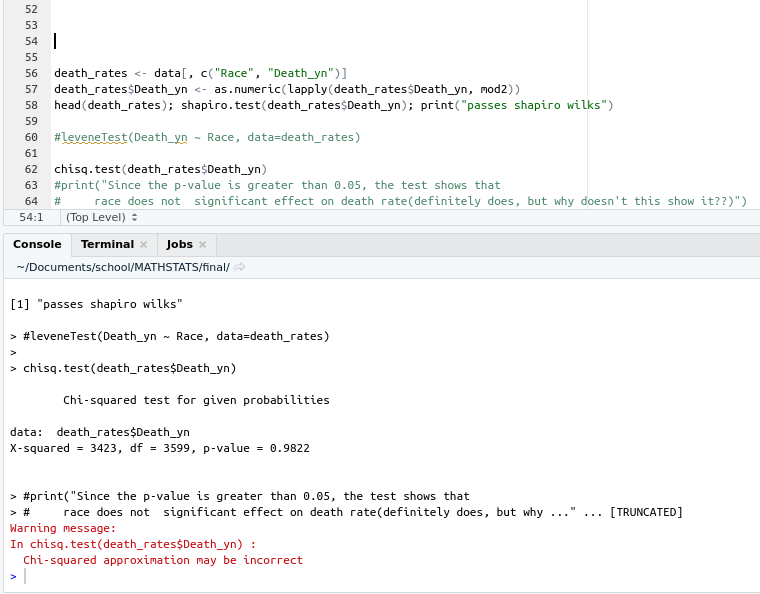
\includegraphics[width=\linewidth]{p2-p2.png}
	\end{figure}
	\item[3.] The population of age 80 or older showed the greatest death rate of the other age groups. 
		After conducting a one-way ANOVA, the resulting p-value was less than 2e-16, which is less than 0.05.
		So, we can reject the null that there is no significant difference between those older than 80 and other age groups.
	\begin{figure}[!h]
		\centering
		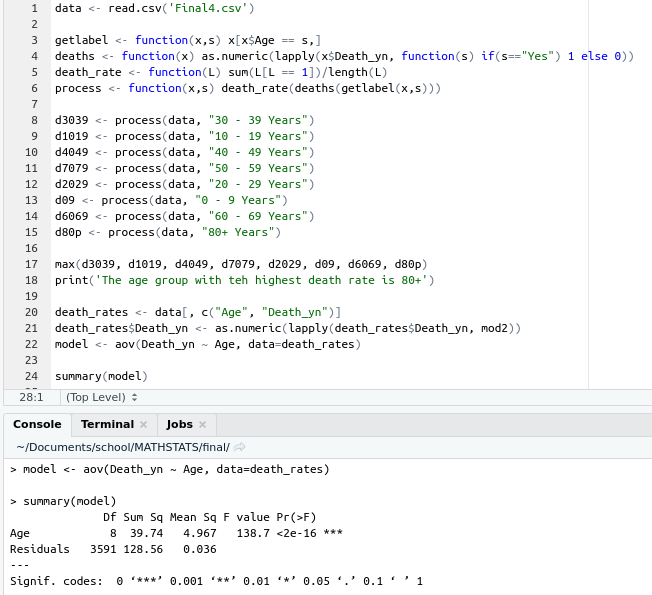
\includegraphics[width=\linewidth]{p3-p.png}
	\end{figure}
	\item[4.] To determine if there is an association between two variables, a Chi-Squared Test of Independence must 
		be conducted. Let the null hypothesis be the claim that seriology level and death rate are independent of 
		each other and the alternative hypothesis that they are associated. After running the ANOVA, the p-value was found to be less than 0.05. So, the null hypothesis is rejected and it can be 
		concluded that there is an association between seriology and death rate. This differs with respect to gender. 
		For if, without loss of generality, the same null and alternative hypotheses are made, the ANOVA
		 reports a p-value greater than 0.05. So, there is no association between gender and death rate.
	\item[5.] Let the null hypothesis claim that there is no association between cholesterol and seriology and the 
		alternative hypothesis claim that there is. Since this implicitly assumes independence, we can proceed 
		with running a Chi-Squared Test of Independence. The test reports a p-value less than 2e-16. So, the null 
		hypothesis is rejected. Therefore, there is an association to be made between cholesterol and death rate.
	\begin{figure}[!h]
		\centering
		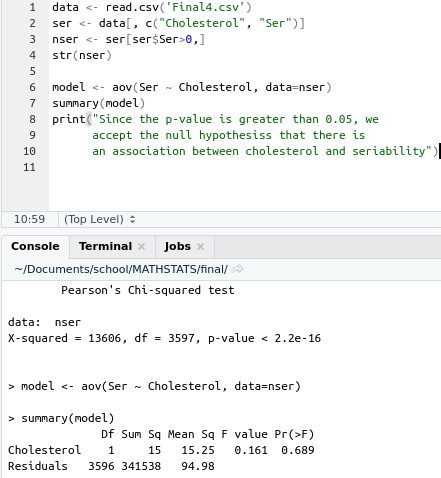
\includegraphics[width=\linewidth]{p5-p2.png}
	\end{figure}
\end{enumerate}

\end{document}
